\documentclass[10pt]{article}
\usepackage{graphicx}
\usepackage[margin=1.5cm]{geometry}
\usepackage{amsmath}
\def\brcurs{{\mbox{$\resizebox{.16in}{.08in}{
\includegraphics{BoldR}}$}}}
\def\rcurs{{\mbox{$\resizebox{.16in}{.08in}{
\includegraphics{ScriptR}}$}}}

\begin{document}
\twocolumn

\title{Tuesday Warm-up: Potentials}
\author{Prof. Jordan C. Hanson}

\maketitle

\section{Memory Bank}

\begin{itemize}
\item \textbf{Fourier series} for a function $f(x)$:
\begin{align}
f(x) &= \frac{A_0}{2} + \sum_{n=1}^{\infty} \left(A_n \cos nx + B_n \sin nx \right) \label{eq:1} \\
A_n &= \frac{1}{\pi}\int_0^{2\pi} f(x) \cos (nx) dx ~~ (n=0,1,2,...) \label{eq:2} \\
B_n &= \frac{1}{\pi}\int_0^{2\pi} f(x) \sin (nx) dx ~~ (n=1,2,...) \label{eq:3}
\end{align}
\item Trigonometric identities:
\begin{align}
\cos\theta\cos\phi &= \frac{1}{2}\left( \cos(\theta - \phi) + \cos(\theta + \phi) \right) \\
\sin\theta\sin\phi &= \frac{1}{2}\left( \cos(\theta - \phi) - \cos(\theta + \phi) \right) \\
\sin\theta\cos\phi &= \frac{1}{2}\left( \sin(\theta + \phi) + \sin(\theta - \phi) \right) \\
\cos\theta\sin\phi &= \frac{1}{2}\left( \sin(\theta + \phi) - \sin(\theta - \phi) \right)
\end{align}
\end{itemize}

\begin{figure}
\centering
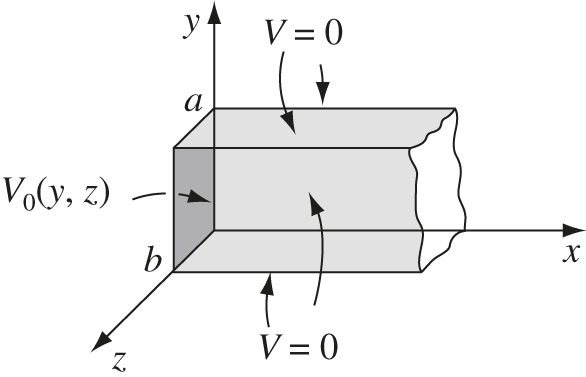
\includegraphics[width=0.33\textwidth]{figures/3_22.jpg}
\caption{\label{fig:1} A waveguide with grounded sides and a potential $V_0(y,z)$ on one side.}
\end{figure}

\section{Separation of Variables}

\begin{enumerate}
\item \textbf{Fourier Series}.  Let $\delta_{nn'} = 1$, if $n=n'$, and $0$ if $n\neq n'$.  (a) Show that the sine functions are \textit{orthogonal}, using an identity in the Memory Bank.  That is, prove that 
\begin{equation}
\int_0^a \sin(n\pi x/a) \sin(n'\pi x/a) dx = \frac{a}{2} \delta_{nn'}
\end{equation}
(b) Create the Fourier series for a square wave.  That is, let $f(x) = 1$ if $0 \leq x \leq \pi$, and $f(x) = 0$ if $\pi \leq x < 2\pi$.  Draw a graph of the \textit{spectrum.}  That is, draw axes labeled \textit{amplitude} versus \textit{frequency}, and make a mark with appropriate height at every frequency in the series. \\ \vspace{5cm}
\item An infinitely long rectangular metal pipe (sides $a$ and $b$) is grounded, but one end, at $x=0$, is maintained at a specified potential $V_0(y,z)$, as indicated in Fig. \ref{fig:1}.  Find the potential inside the pipe.
\begin{itemize}
\item Write the six boundary conditions as equations: \\ \vspace{1cm}
\item Write the solution as $v(x,y,z) = X(x) Y(y) Z(z)$, and separate the variables. \\ \vspace{2cm}
\item Set the ordinary $X$, $Y$, and $Z$ differential equations equal to constants that sum to zero. \\ \vspace{1cm}
\item Show that the specific solution is proportional to a decaying exponential in $x$, and the product of sine functions in $y$ and $z$.
\end{itemize}
\end{enumerate}

\end{document}
